\documentclass{standalone}
\usepackage{tikz}
\usetikzlibrary{patterns, positioning}

\begin{document}
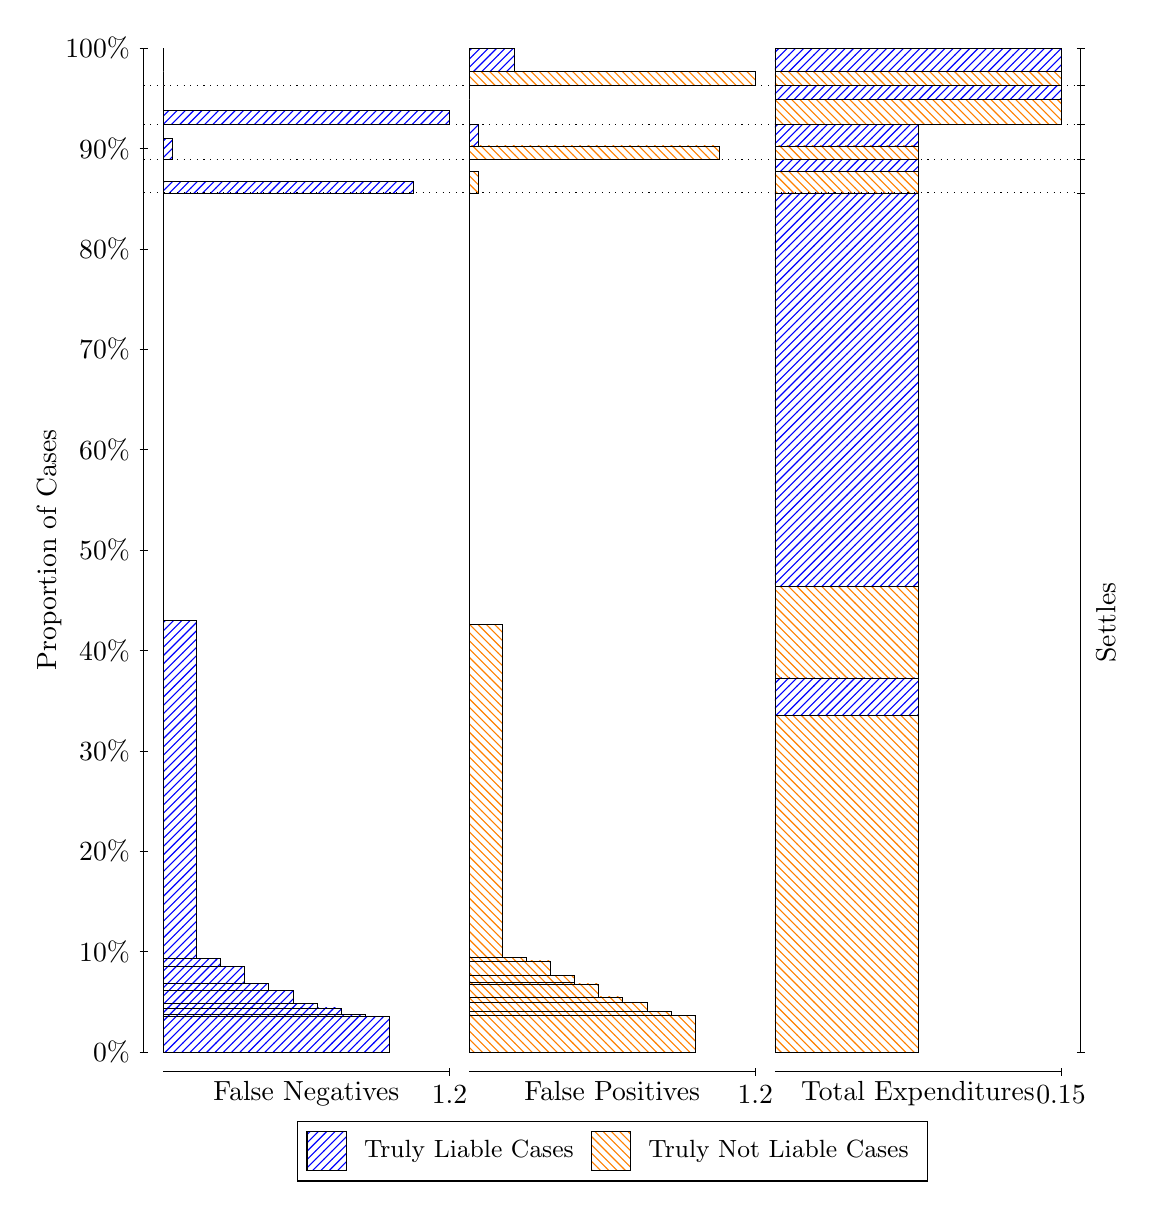
\begin{tikzpicture}
\draw[black, very thin] (1.5,1.75) -- (1.5,14.5);
\node[rotate=90, anchor=center] at (0.3, 8.125) {Proportion of Cases};
\draw[black, very thin] (1.45,1.75) -- (1.55,1.75);
\node[anchor=east] at (1.45, 1.75) {0\%};
\draw[black, very thin] (1.45,3.025) -- (1.55,3.025);
\node[anchor=east] at (1.45, 3.025) {10\%};
\draw[black, very thin] (1.45,4.3) -- (1.55,4.3);
\node[anchor=east] at (1.45, 4.3) {20\%};
\draw[black, very thin] (1.45,5.575) -- (1.55,5.575);
\node[anchor=east] at (1.45, 5.575) {30\%};
\draw[black, very thin] (1.45,6.85) -- (1.55,6.85);
\node[anchor=east] at (1.45, 6.85) {40\%};
\draw[black, very thin] (1.45,8.125) -- (1.55,8.125);
\node[anchor=east] at (1.45, 8.125) {50\%};
\draw[black, very thin] (1.45,9.4) -- (1.55,9.4);
\node[anchor=east] at (1.45, 9.4) {60\%};
\draw[black, very thin] (1.45,10.675) -- (1.55,10.675);
\node[anchor=east] at (1.45, 10.675) {70\%};
\draw[black, very thin] (1.45,11.95) -- (1.55,11.95);
\node[anchor=east] at (1.45, 11.95) {80\%};
\draw[black, very thin] (1.45,13.225) -- (1.55,13.225);
\node[anchor=east] at (1.45, 13.225) {90\%};
\draw[black, very thin] (1.45,14.5) -- (1.55,14.5);
\node[anchor=east] at (1.45, 14.5) {100\%};

\draw[black, very thin] (13.4,1.75) -- (13.4,14.5);
\draw[black, very thin] (13.35,1.75) -- (13.45,1.75);
\node[anchor=west] at (13.35, 1.75) {};
\draw[black, very thin] (13.35,12.661) -- (13.45,12.661);
\node[anchor=west] at (13.35, 12.661) {};
\draw[black, very thin] (13.35,13.082) -- (13.45,13.082);
\node[anchor=west] at (13.35, 13.082) {};
\draw[black, very thin] (13.35,13.527) -- (13.45,13.527);
\node[anchor=west] at (13.35, 13.527) {};
\draw[black, very thin] (13.35,14.026) -- (13.45,14.026);
\node[anchor=west] at (13.35, 14.026) {};
\draw[black, very thin] (13.35,14.5) -- (13.45,14.5);
\node[anchor=west] at (13.35, 14.5) {};

\draw[black, very thin, pattern color=blue, pattern=north east lines] (1.75,1.75) rectangle (4.6184,2.2069);
\draw[black, very thin, pattern color=blue, pattern=north east lines] (1.75,2.2069) rectangle (4.3125,2.2247);
\draw[black, very thin, pattern color=blue, pattern=north east lines] (1.75,2.2247) rectangle (4.0065,2.3086);
\draw[black, very thin, pattern color=blue, pattern=north east lines] (1.75,2.3086) rectangle (3.7005,2.3701);
\draw[black, very thin, pattern color=blue, pattern=north east lines] (1.75,2.3701) rectangle (3.3946,2.5325);
\draw[black, very thin, pattern color=blue, pattern=north east lines] (1.75,2.5325) rectangle (3.0886,2.6251);
\draw[black, very thin, pattern color=blue, pattern=north east lines] (1.75,2.6251) rectangle (2.7826,2.8384);
\draw[black, very thin, pattern color=blue, pattern=north east lines] (1.75,2.8384) rectangle (2.4767,2.9421);
\draw[black, very thin, pattern color=blue, pattern=north east lines] (1.75,2.9421) rectangle (2.1707,7.2269);
\draw[black, very thin, pattern color=orange, pattern=north west lines] (1.75,7.2269) rectangle (1.75,12.661);
\draw[black, very thin, pattern color=blue, pattern=north east lines] (1.75,12.661) rectangle (4.9244,12.81);
\draw[black, very thin, pattern color=orange, pattern=north west lines] (1.75,12.81) rectangle (1.75,13.082);
\draw[black, very thin, pattern color=blue, pattern=north east lines] (1.75,13.082) rectangle (1.8647,13.353);
\draw[black, very thin, pattern color=orange, pattern=north west lines] (1.75,13.353) rectangle (1.75,13.527);
\draw[black, very thin, pattern color=blue, pattern=north east lines] (1.75,13.527) rectangle (5.3833,13.706);
\draw[black, very thin, pattern color=orange, pattern=north west lines] (1.75,13.706) rectangle (1.75,14.026);
\draw[black, very thin, pattern color=orange, pattern=north west lines] (1.75,14.026) rectangle (1.75,14.202);
\draw[black, very thin, pattern color=blue, pattern=north east lines] (1.75,14.202) rectangle (1.75,14.5);
\draw[black, very thin, pattern color=orange, pattern=north west lines] (5.6333,1.75) rectangle (8.5018,2.2155);
\draw[black, very thin, pattern color=orange, pattern=north west lines] (5.6333,2.2155) rectangle (8.1958,2.2616);
\draw[black, very thin, pattern color=orange, pattern=north west lines] (5.6333,2.2616) rectangle (7.8898,2.3758);
\draw[black, very thin, pattern color=orange, pattern=north west lines] (5.6333,2.3758) rectangle (7.5839,2.4502);
\draw[black, very thin, pattern color=orange, pattern=north west lines] (5.6333,2.4502) rectangle (7.2779,2.6136);
\draw[black, very thin, pattern color=orange, pattern=north west lines] (5.6333,2.6136) rectangle (6.9719,2.6371);
\draw[black, very thin, pattern color=orange, pattern=north west lines] (5.6333,2.6371) rectangle (6.9719,2.7244);
\draw[black, very thin, pattern color=orange, pattern=north west lines] (5.6333,2.7244) rectangle (6.666,2.9077);
\draw[black, very thin, pattern color=orange, pattern=north west lines] (5.6333,2.9077) rectangle (6.36,2.948);
\draw[black, very thin, pattern color=orange, pattern=north west lines] (5.6333,2.948) rectangle (6.054,7.1837);
\draw[black, very thin, pattern color=blue, pattern=north east lines] (5.6333,7.1837) rectangle (5.6333,12.661);
\draw[black, very thin, pattern color=orange, pattern=north west lines] (5.6333,12.661) rectangle (5.7481,12.933);
\draw[black, very thin, pattern color=blue, pattern=north east lines] (5.6333,12.933) rectangle (5.6333,13.082);
\draw[black, very thin, pattern color=orange, pattern=north west lines] (5.6333,13.082) rectangle (8.8077,13.256);
\draw[black, very thin, pattern color=blue, pattern=north east lines] (5.6333,13.256) rectangle (5.7481,13.527);
\draw[black, very thin, pattern color=orange, pattern=north west lines] (5.6333,13.527) rectangle (5.6333,13.847);
\draw[black, very thin, pattern color=blue, pattern=north east lines] (5.6333,13.847) rectangle (5.6333,14.026);
\draw[black, very thin, pattern color=orange, pattern=north west lines] (5.6333,14.026) rectangle (9.2667,14.202);
\draw[black, very thin, pattern color=blue, pattern=north east lines] (5.6333,14.202) rectangle (6.207,14.5);
\draw[black, very thin, pattern color=orange, pattern=north west lines] (9.5167,1.75) rectangle (11.333,6.026);
\draw[black, very thin, pattern color=blue, pattern=north east lines] (9.5167,6.026) rectangle (11.333,6.5007);
\draw[black, very thin, pattern color=orange, pattern=north west lines] (9.5167,6.5007) rectangle (11.333,7.6584);
\draw[black, very thin, pattern color=blue, pattern=north east lines] (9.5167,7.6584) rectangle (11.333,12.661);
\draw[black, very thin, pattern color=orange, pattern=north west lines] (9.5167,12.661) rectangle (11.333,12.933);
\draw[black, very thin, pattern color=blue, pattern=north east lines] (9.5167,12.933) rectangle (11.333,13.082);
\draw[black, very thin, pattern color=orange, pattern=north west lines] (9.5167,13.082) rectangle (11.333,13.256);
\draw[black, very thin, pattern color=blue, pattern=north east lines] (9.5167,13.256) rectangle (11.333,13.527);
\draw[black, very thin, pattern color=orange, pattern=north west lines] (9.5167,13.527) rectangle (13.15,13.847);
\draw[black, very thin, pattern color=blue, pattern=north east lines] (9.5167,13.847) rectangle (13.15,14.026);
\draw[black, very thin, pattern color=orange, pattern=north west lines] (9.5167,14.026) rectangle (13.15,14.202);
\draw[black, very thin, pattern color=blue, pattern=north east lines] (9.5167,14.202) rectangle (13.15,14.5);
\draw[black, dotted] (1.5,12.661) -- (13.4,12.661);
\draw[black, dotted] (1.5,13.082) -- (13.4,13.082);
\draw[black, dotted] (1.5,13.527) -- (13.4,13.527);
\draw[black, dotted] (1.5,14.026) -- (13.4,14.026);
\draw[black, very thin] (1.75,1.5) -- (5.3833,1.5);
\node[anchor=north] at (3.5667, 1.5) {False Negatives};
\draw[black, very thin] (5.3833,1.45) -- (5.3833,1.55);
\node[anchor=north] at (5.3833, 1.45) {1.2};

\draw[black, very thin] (5.6333,1.5) -- (9.2667,1.5);
\node[anchor=north] at (7.45, 1.5) {False Positives};
\draw[black, very thin] (9.2667,1.45) -- (9.2667,1.55);
\node[anchor=north] at (9.2667, 1.45) {1.2};

\draw[black, very thin] (9.5167,1.5) -- (13.15,1.5);
\node[anchor=north] at (11.333, 1.5) {Total Expenditures};
\draw[black, very thin] (13.15,1.45) -- (13.15,1.55);
\node[anchor=north] at (13.15, 1.45) {0.15};

\node[black, centered, rotate=90] at (13.72, 7.2053) {Settles};





\draw (7.449999999999999,1.5) node[draw=none] (baseCoordinate) {};
\begin{scope}[align=center]
        \matrix[scale=0.5, draw=black, below=0.5cm of baseCoordinate, nodes={draw}, column sep=0.1cm]{
            \node[rectangle, draw, minimum width=0.5cm, minimum height=0.5cm, pattern=north east lines, pattern color=blue] {}; &
            \node[draw=none, font=\small] (B) {Truly Liable Cases}; &
            \node[rectangle, draw, minimum width=0.5cm, minimum height=0.5cm, pattern=north west lines, pattern color=orange] {}; &
            \node[draw=none, font=\small] (B) {Truly Not Liable Cases}; \\
            };
\end{scope}

\end{tikzpicture}
\end{document}